\documentclass[leqno, letterpaper, 11pt]{article}
\usepackage{amssymb}
\usepackage{amsmath}
\usepackage{tikz}
\usetikzlibrary{through,calc,positioning,decorations.pathreplacing}

\begin{document}

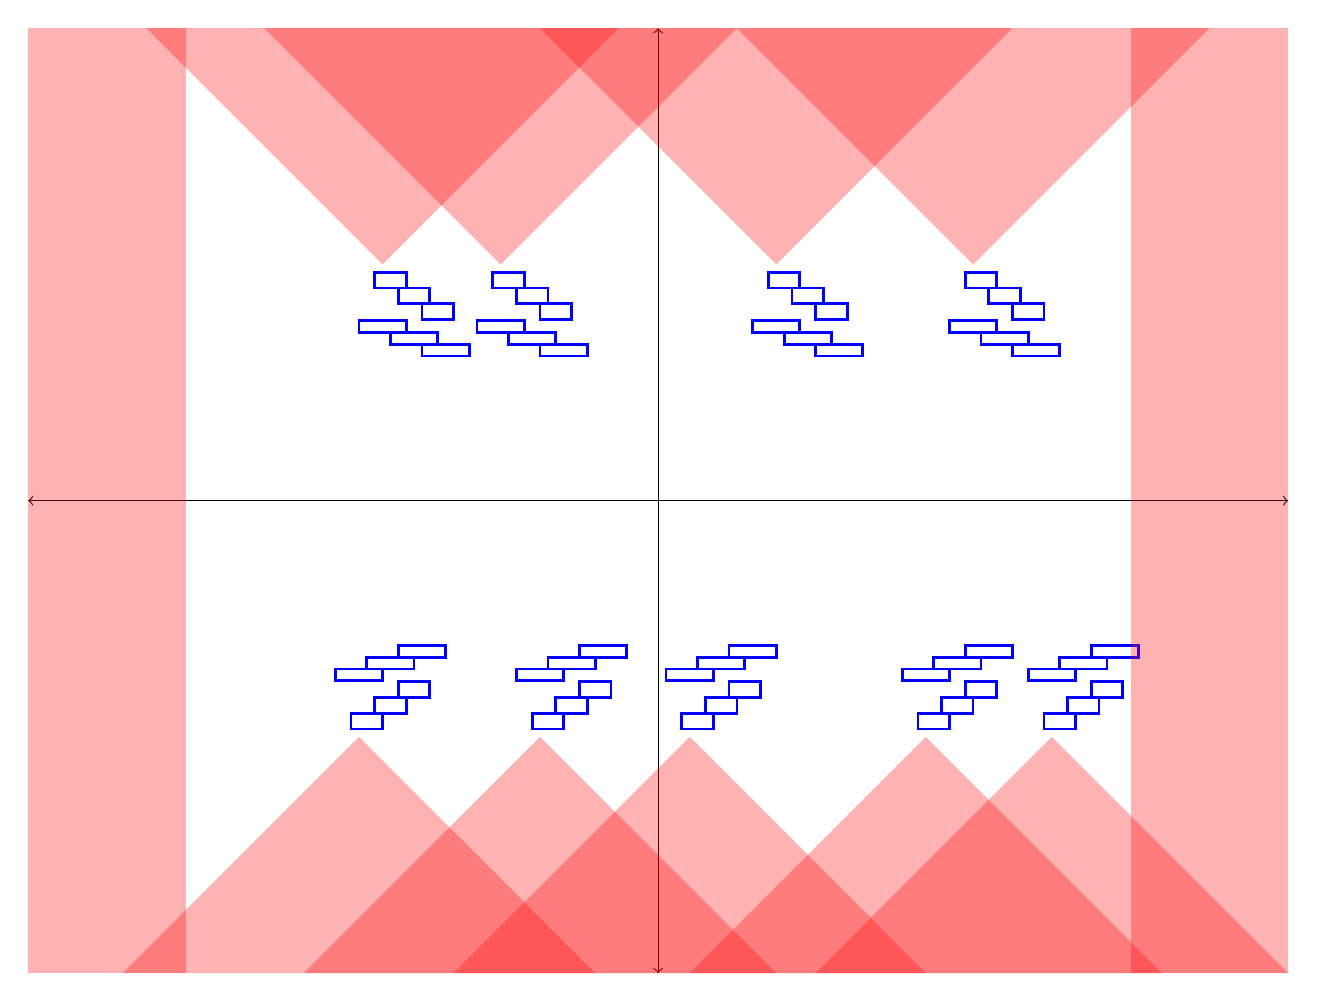
\begin{tikzpicture}



\def\a{1}
\def\f{4}
\def\m{3}

\pgfmathsetmacro\l{{(\m+\a*\m-1)/(\m+1)}}
\pgfmathsetmacro\s{{2*\m*sqrt(\l)/(sqrt(\l)-1}}
\pgfmathsetmacro\g{{\a*\f/2}};
\pgfmathsetmacro\h{{(\m*\g-\f)/(\m+1)}}
\pgfmathsetmacro\fp{\l*\f}
\pgfmathsetmacro\hp{\l*\h}
\pgfmathsetmacro\gp{\l*\g}

\draw[color=black, <->] (-8,0)--(8,0);
\draw[color=black, <->] (0, -6)--(0,6);

\foreach \k in {-3.8,-1.5,0.4,3.4,5}
{
\fill[opacity=0.3,red]{(\k-3,-6)--(\k, -3)--(\k+3,-6)};
 
\foreach \i in {1,...,\m}
{
 \draw[color=blue, line width=1] ({(\i-1)*0.4-\i*0.1+\k},\i*0.2-3-0.1) rectangle ({\i*0.4-\i*0.1+\k},\i*0.2-3+0.1);

\draw[color=blue, line width=1] 
({(\i-1)*0.6-\i*0.2+\k-0.1},\m*0.2+\i*0.15-3-0.075+0.075/2) rectangle ({\i*0.6-\i*0.2+\k-0.1},\m*0.2+\i*0.15-3+0.075+0.075/2);
} 
}

\foreach \k in {-3.5,-2,1.5,4}
{
\fill[opacity=0.3,red]{(\k-3,6)--(\k, 3)--(\k+3,6)};
 
\foreach \i in {1,...,\m}{
 
    \draw[color=blue, line width=1] 
    ({(\i-1)*0.4-\i*0.1+\k},-\i*0.2+3+0.1) rectangle ({\i*0.4-\i*0.1+\k},-\i*0.2+3-0.1);
  
    \draw[color=blue, line width=1] ({(\i-1)*0.6-\i*0.2+\k-0.1},-\m*0.2-\i*0.15+3+0.075-0.075/2) rectangle ({\i*0.6-\i*0.2+\k-0.1},-\m*0.2-\i*0.15+3-0.075-0.075/2);
}    
}

\fill[opacity=0.3,red] (-8,-6) rectangle (-6,6);
\fill[opacity=0.3,red] (6,-6) rectangle (8,6);
  
\end{tikzpicture}

\end{document}